\section{Supplementary Material}

\begin{figure}
    \begin{center}
        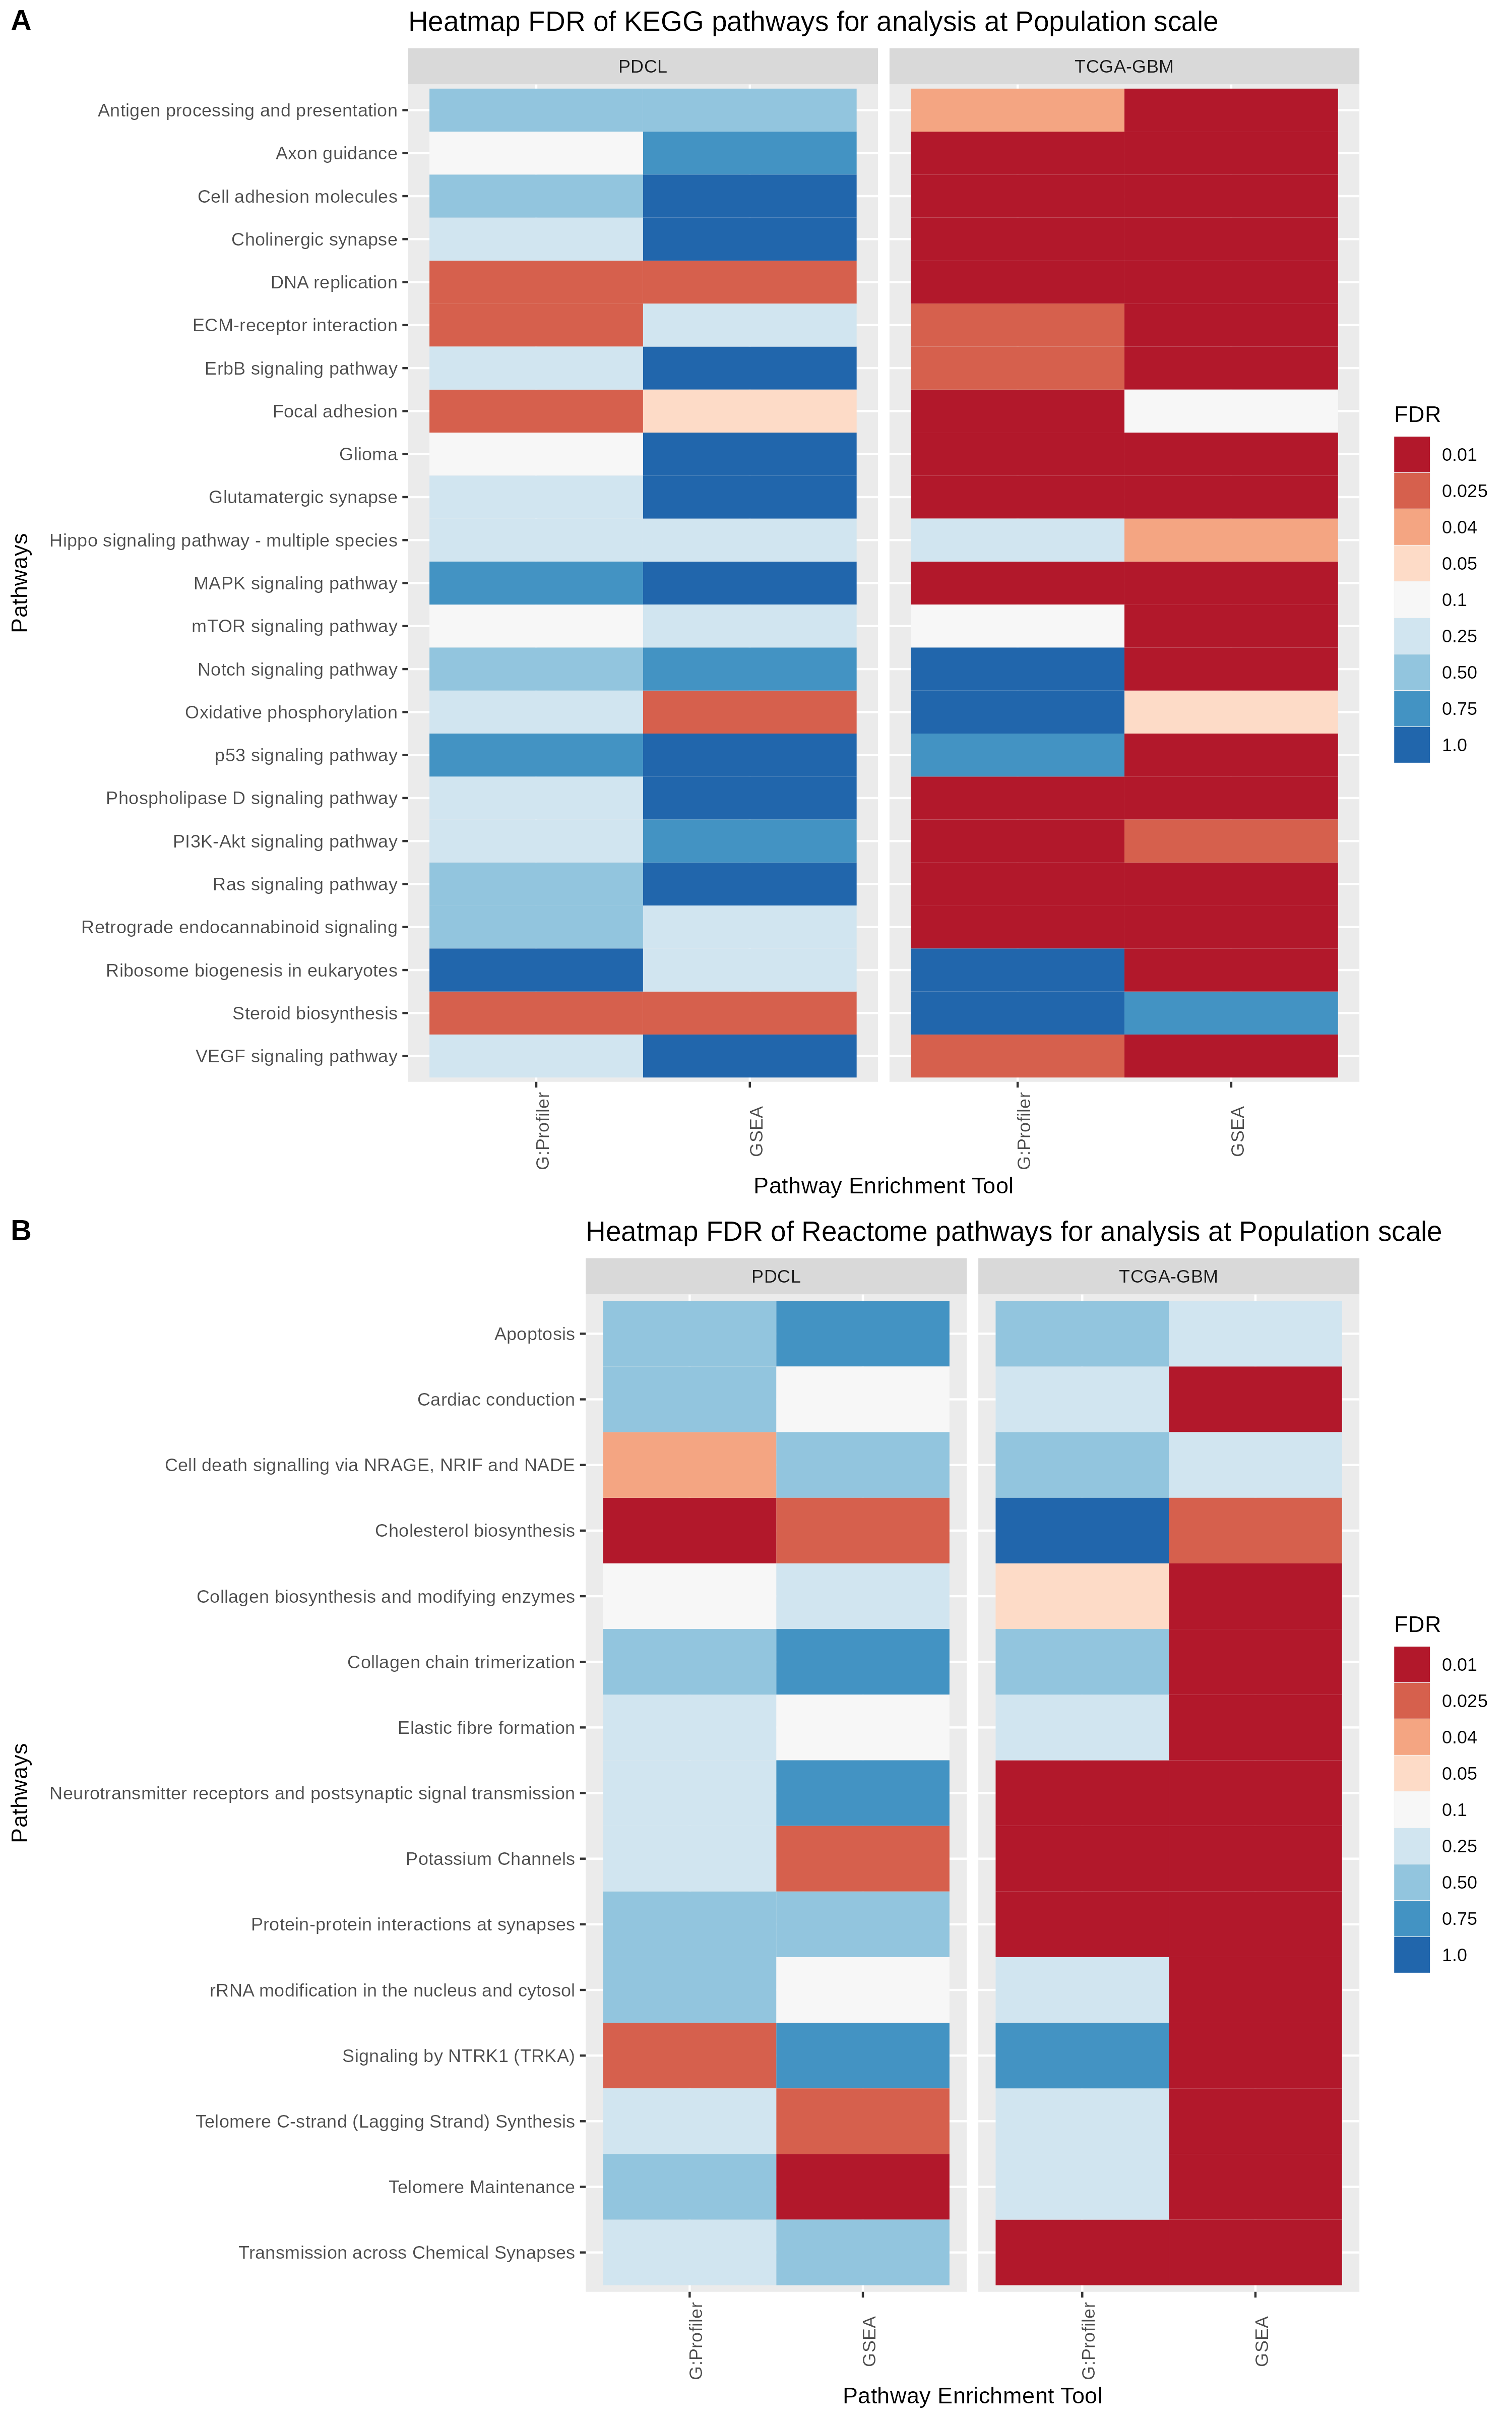
\includegraphics[height=0.7\paperheight]{img/heatmap-fdr-global}
        \caption{
            Heatmap of deregulated pathways in the \acrshort{pdcl} and the \acrshort{tcga} datasets for (A) the \acrshort{kegg} database and (B) the Reactome database.
            \acrshort{fdr} values below 5\% are considered significant (red) and their are not considered significant if greater than 5\% (blue).
        }
        \label{supp:heatmap-fdr-global}
    \end{center}
\end{figure}


\begin{figure}
    \begin{center}
        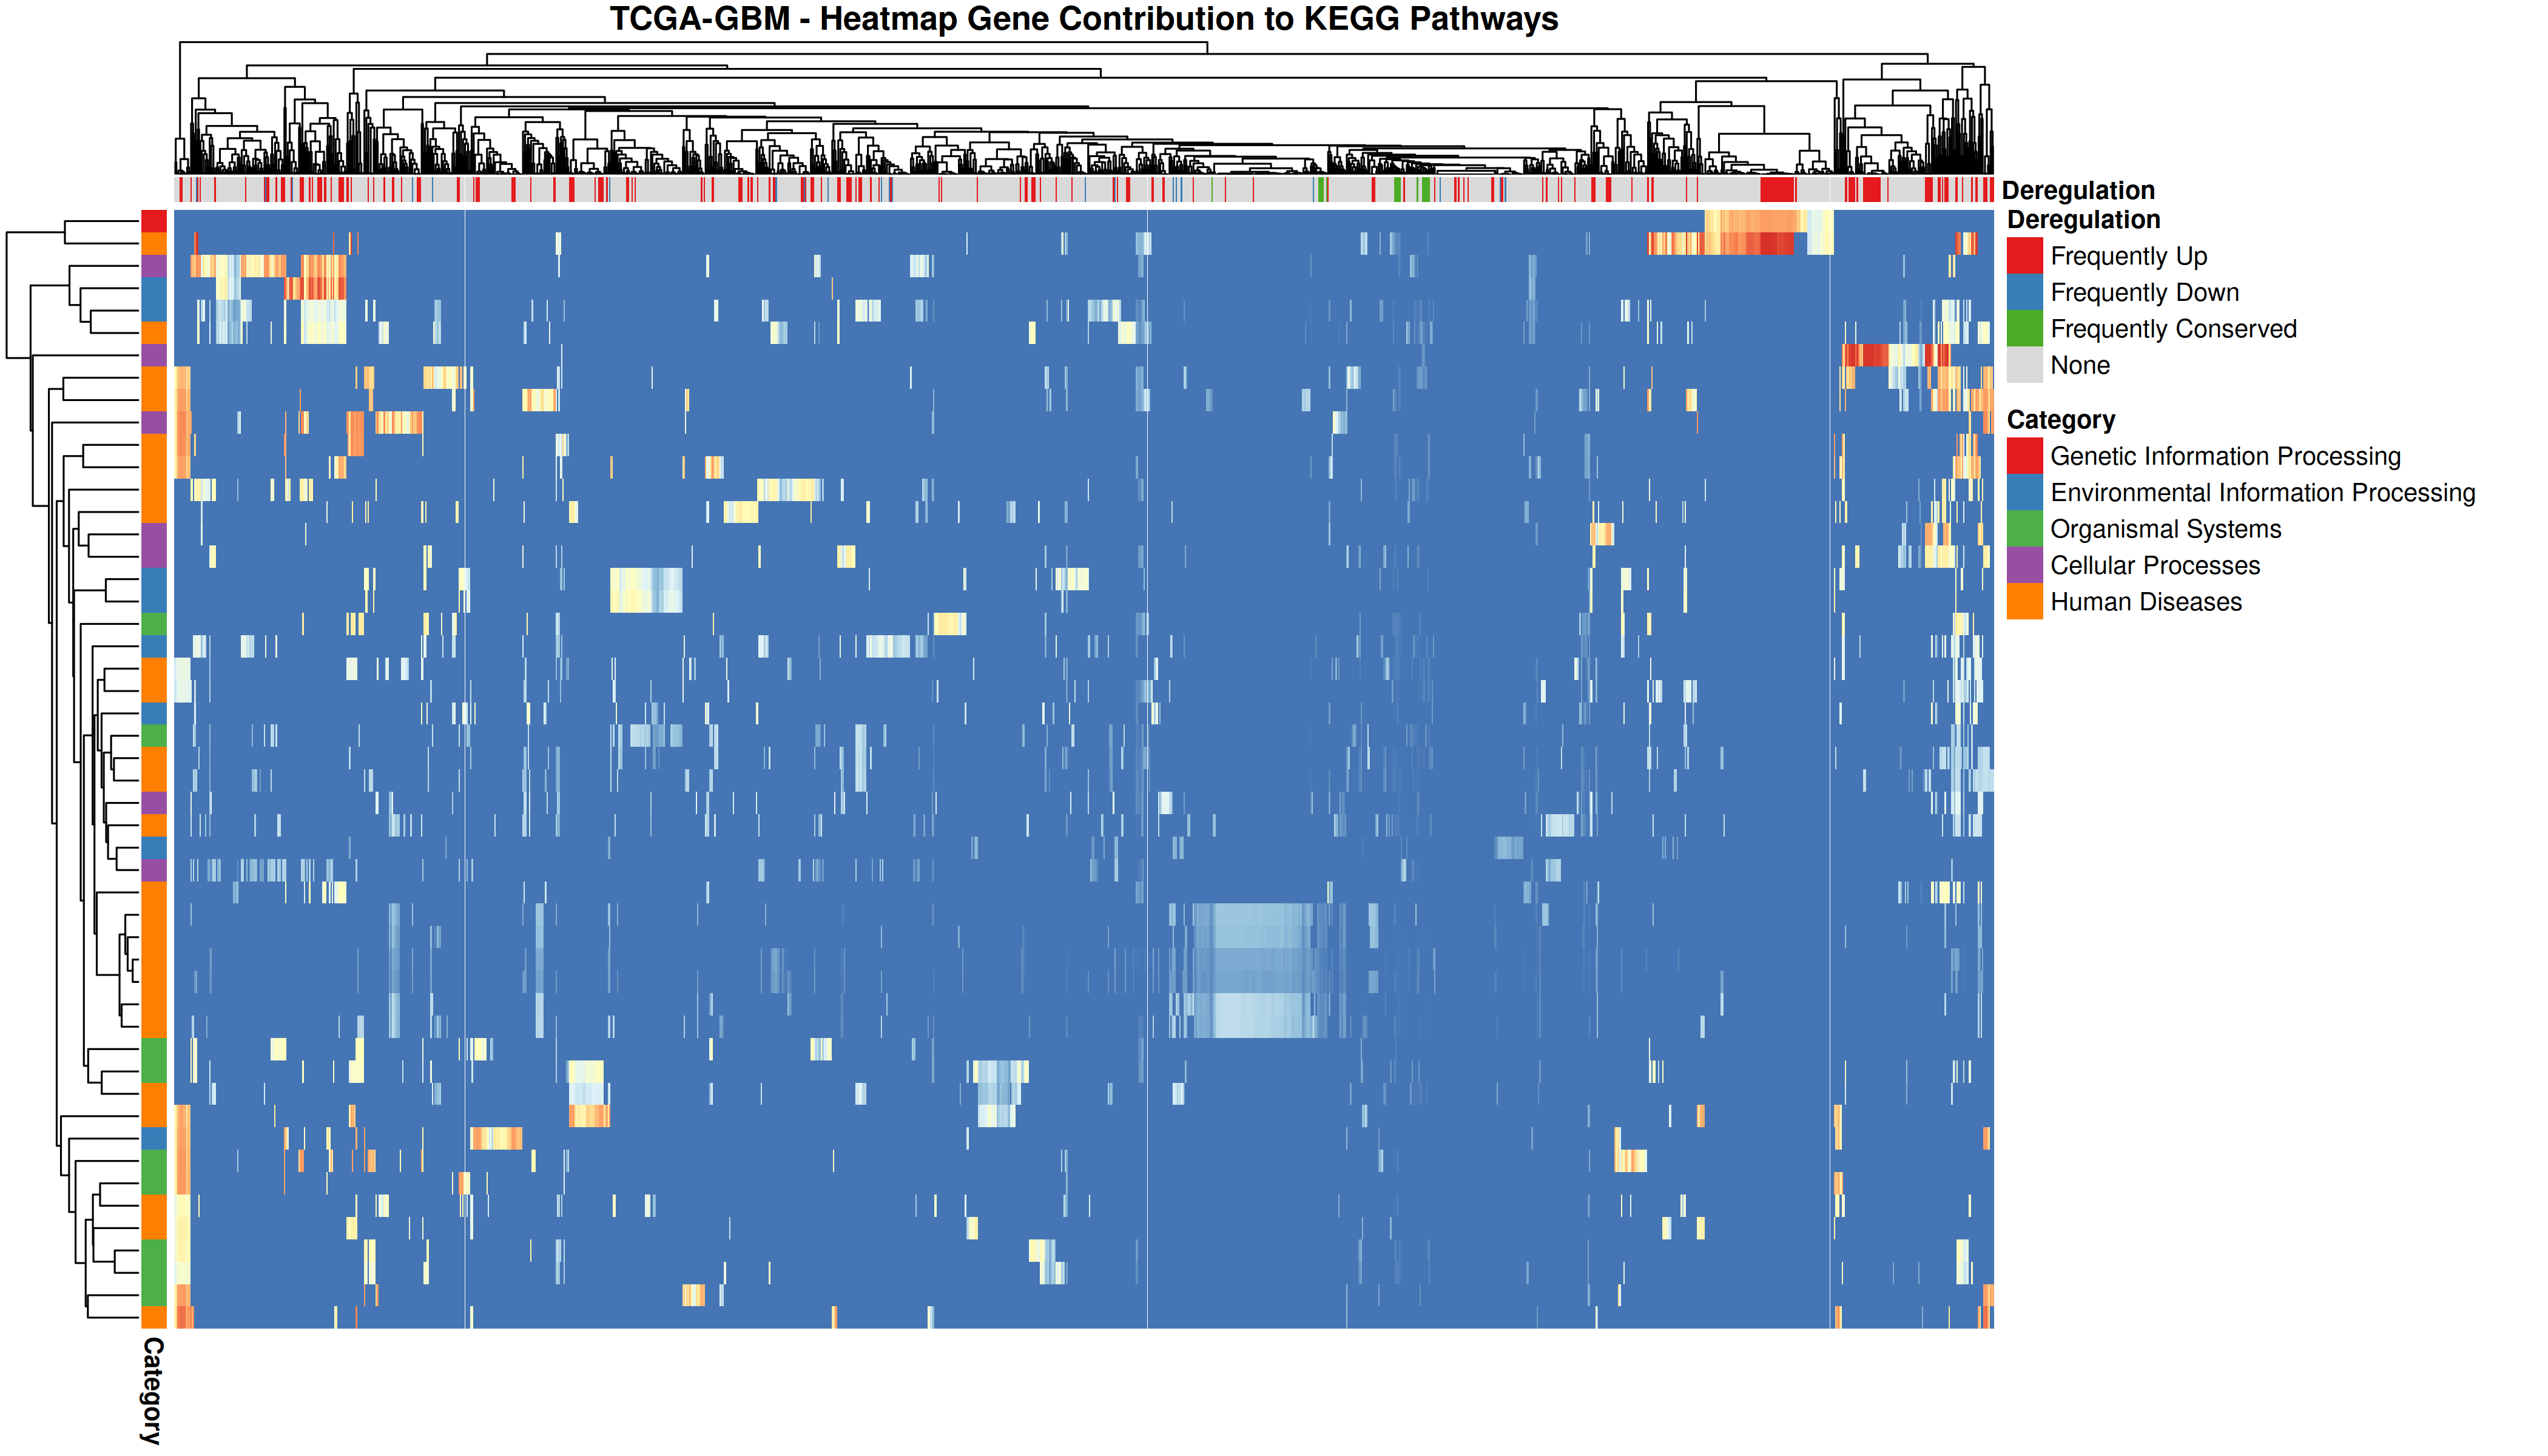
\includegraphics[width=\textwidth]{img/gene_contrib_kegg_tcga}
        \caption {
            Heatmap of the gene contributions for each pathways with \acrshort{tcga} data and \acrshort{kegg} categories.
            Genes contribution to a pathway is computed by calculating how many times a gene appear in the enrichment result for a pathway.
            Red colour indicate a strong contribution and blue colour indicate a week contribution.
            Only genes with a total contributions higher than the third quartile and pathways where the total gene contribution is higher than the third quartile are kept.
            Pathways are colored by their categories.
            Genes are colored by their deregulation frequency : red indicate genes that are up-regulated in 90\% of the samples, blue indicate genes that are down-regulated in 90\% of the samples, green indicate genes that are not deregulated in 90\% of the samples and grey genes that correspond to none of the above.
        }
        \label{supp:gene-contrib-kegg-tcga}
    \end{center}
\end{figure}

\begin{figure}
    \begin{center}
        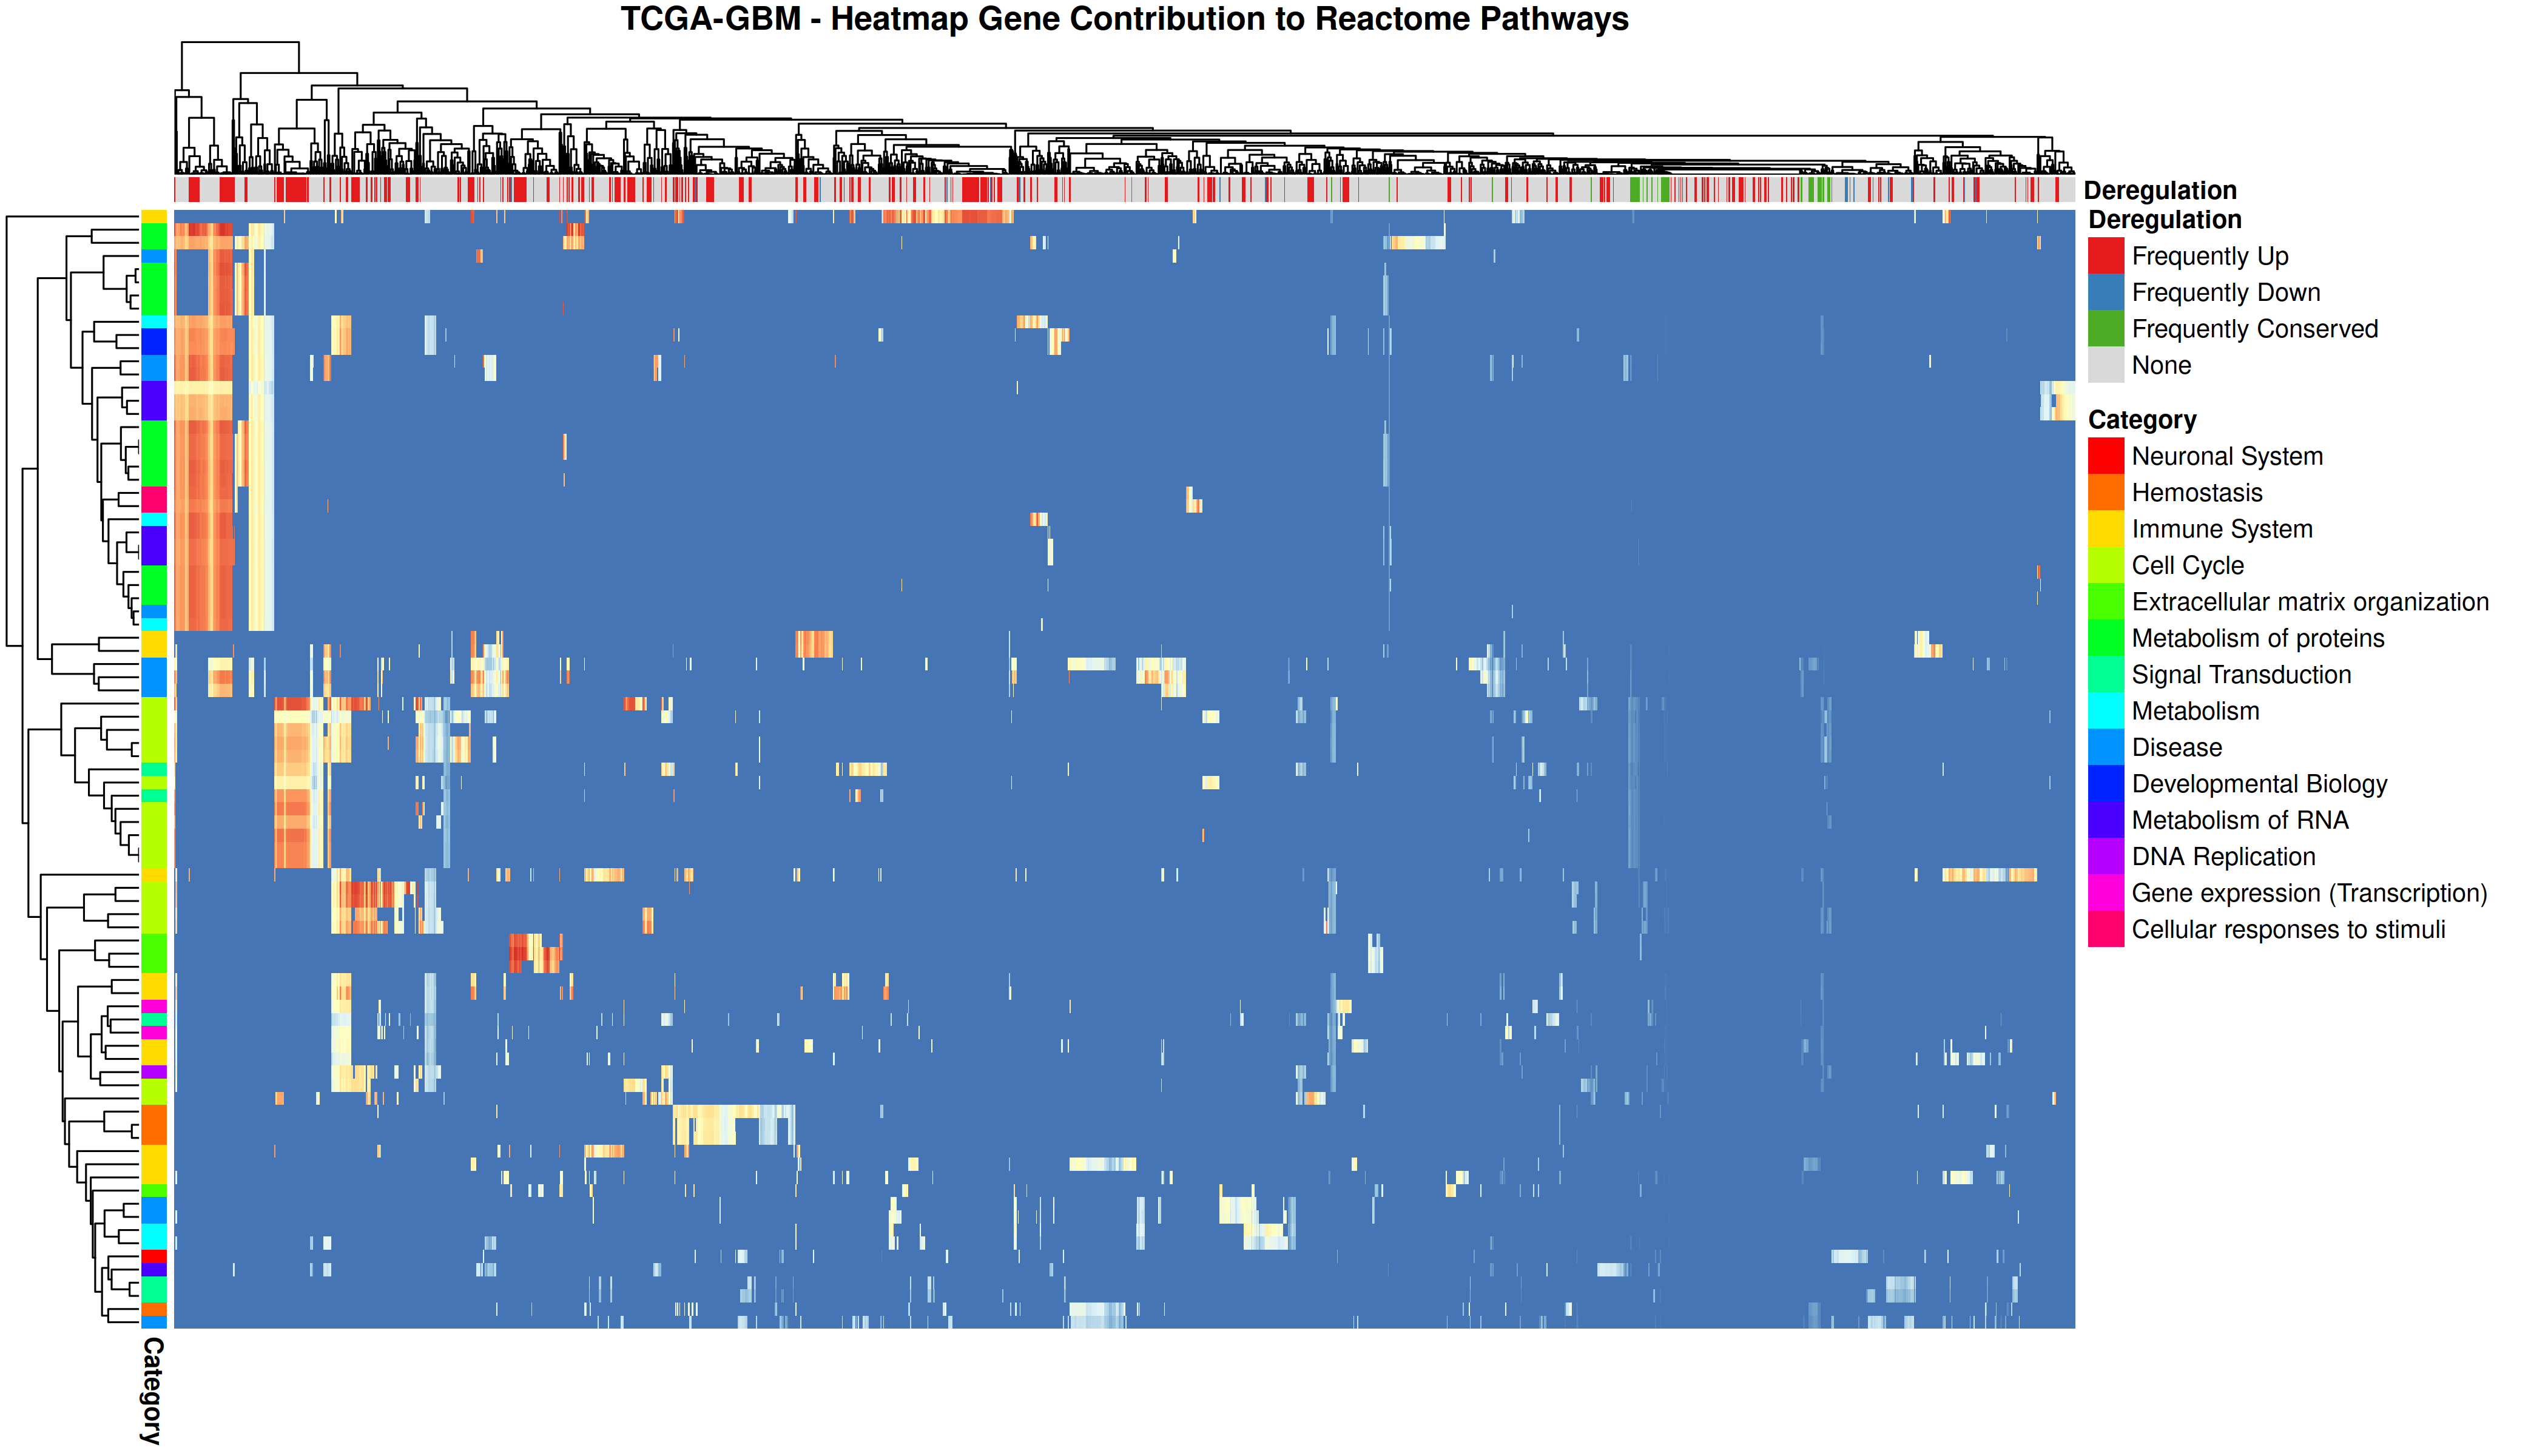
\includegraphics[width=\textwidth]{img/gene_contrib_reactome_tcga}
        \caption {
            Heatmap of the gene contributions for each pathways with \acrshort{tcga} data and Reactome categories.
            Genes contribution to a pathway is computed by calculating how many times a gene appear in the enrichment result for a pathway.
            Red colour indicate a strong contribution and blue colour indicate a week contribution.
            Only genes with a total contributions higher than the 90\% percentile and pathways where the total gene contribution is higher than the third quartile are kept.
            Pathways are colored by their categories.
            Genes are colored by their deregulation frequency : red indicate genes that are up-regulated in 90\% of the samples, blue indicate genes that are down-regulated in 90\% of the samples, green indicate genes that are not deregulated in 90\% of the samples and grey genes that correspond to none of the above.
        }
        \label{supp:gene-contrib-reactome-tcga}
    \end{center}
\end{figure}